\documentclass[9pt]{beamer}

\usepackage[utf8x]{inputenc}
\usepackage[english]{babel}
\usepackage{amsmath, amsfonts, amssymb}
\usepackage{color}
\usepackage{xcolor}
\usepackage{tikz}
\usetikzlibrary{positioning,shapes,shadows,arrows,snakes}
\usepackage{listliketab}
\usepackage{shuffle}
\usepackage{xargs}
\usepackage{multirow}
\usepackage{pgfplots}
\usepackage{csquotes}
\usepackage{verbatim}

\definecolor{BlueGreen}{cmyk}{0.85,0,0.33,0}
\definecolor{RawSienna}{cmyk}{0,0.72,1,0.45}
\definecolor{gold}{rgb}{1.,0.84,0.}
\definecolor{dgreen}{rgb}{0.,0.6,0.}

\definecolor{Noir}{RGB}{0,0,0}
\definecolor{Rouge}{RGB}{205,35,38}
\definecolor{Bleu}{RGB}{2,60,195}
\definecolor{Bleu1}{RGB}{121,176,197}
\definecolor{Vert}{RGB}{23,103,1}
\definecolor{VertOlive}{RGB}{112,141,35}
\definecolor{Orange}{RGB}{255,113,15}
\definecolor{RoseBonbon}{RGB}{249,66,158}
\definecolor{Marron}{RGB}{193,88,50}

\definecolor{mygreen}{RGB}{23,103,1}

\newcommand{\red}[1]{\textcolor{red}{#1}}
\newcommand{\blue}[1]{\textcolor{blue}{#1}}
\newcommand{\green}[1]{\textcolor{mygreen}{#1}}
\newcommand{\bluealert}[2]{\textcolor<#1>{blue}{#2}}

\tikzstyle{alert} = [color=red, line width = 1.5]
\tikzstyle{bluealert} = [color=blue, line width =1.5]
\tikzstyle{big} = [line width = 1.5]
\tikzstyle{Point} = [fill, radius=0.08]
\tikzstyle{RedPoint} = [fill, radius=0.09, color = red]


\tikzstyle{Red} = [color = red]
\tikzstyle{Blue} = [color = blue]
\tikzstyle{Green} = [color = Vert]
\tikzstyle{Gray} = [color = gray]

\definecolor{violet}{rgb}{.5,.1,.9}

\input{commands.tex}

\usetheme{Boadilla}
\title{Transfer learning with Transformer networks}
\author[G. Châtel]{Grégory Châtel\\\vspace{0.3cm}Disaitek\\Intel Software Innovator\\\vspace{0.3cm}@rodgzilla\\github.com/rodgzilla}
\date{11/28/2018}

\setbeamertemplate{footline}[frame number]{}
\setbeamertemplate{navigation symbols}{}
%% \setbeamertemplate{footline}[frame number]{}


\begin{document}

%%%%%%%%%%%%%%%%%%%%%%%%%%%%%%%%%%%%%%%%%%%%%%%%%%%%%%%%%%%%%%%%%%%%%%
\begin{frame}

  \maketitle

\end{frame}
%%%%%%%%%%%%%%%%%%%%%%%%%%%%%%%%%%%%%%%%%%%%%%%%%%%%%%%%%%%%%%%%%%%%%%

\section{Introduction}

%%%%%%%%%%%%%%%%%%%%%%%%%%%%%%%%%%%%%%%%%%%%%%%%%%%%%%%%%%%%%%%%%%%%%%
\begin{frame}

  \frametitle{Neural network architectures for NLP}


  MLP, CNN, dilated CNN, RNN (LSTM / GRU), Tranformer
\end{frame}
%%%%%%%%%%%%%%%%%%%%%%%%%%%%%%%%%%%%%%%%%%%%%%%%%%%%%%%%%%%%%%%%%%%%%%

%%%%%%%%%%%%%%%%%%%%%%%%%%%%%%%%%%%%%%%%%%%%%%%%%%%%%%%%%%%%%%%%%%%%%%
\begin{frame}

  \frametitle{Attention mechanisms}

  \framesubtitle{Scaled Dot-Product Attention}

  \begin{figure}
    \includegraphics[height = 3.5cm]{images/dot_product_attention.png}
  \end{figure}

  \medskip

  $Q$ is the query vector, $K$ is the key vector and $V$ value vector.

  \bigskip

  \[
  \text{Attention}(Q, K, V) = \text{softmax}(\frac{QK^{T}}{\sqrt{d_{k}}}) V.
  \]

\end{frame}
%%%%%%%%%%%%%%%%%%%%%%%%%%%%%%%%%%%%%%%%%%%%%%%%%%%%%%%%%%%%%%%%%%%%%%

%%%%%%%%%%%%%%%%%%%%%%%%%%%%%%%%%%%%%%%%%%%%%%%%%%%%%%%%%%%%%%%%%%%%%%
\begin{frame}

  \frametitle{Attention mechanisms}

  \framesubtitle{Multi-Head Attention}

  \begin{figure}
    \includegraphics[height = 4cm]{images/multi_head_attention.png}
  \end{figure}

  \begin{align*}
    \text{MultiHead}(Q, K, V) &= \text{Concat}(\text{head}_{1}, \dots, \text{head}_{h}) \\
    \text{where} \quad \text{head}_{i} &= \text{Attention}(QW^{Q}_{i}, KW^{K}_{i},
  VW^{V}_{i})
  \end{align*}

  \bigskip

  where the projections $W^{Q}_{i}$, $W^{K}_{i}$ and $W^{V}_{i}$ are
  parameter matrices.
\end{frame}
%%%%%%%%%%%%%%%%%%%%%%%%%%%%%%%%%%%%%%%%%%%%%%%%%%%%%%%%%%%%%%%%%%%%%%

%%%%%%%%%%%%%%%%%%%%%%%%%%%%%%%%%%%%%%%%%%%%%%%%%%%%%%%%%%%%%%%%%%%%%%
\begin{frame}

  \frametitle{Transformer network}

  \framesubtitle{Original transformer}

  \begin{figure}
    \includegraphics[width = 5cm]{images/base_transformer.png}
  \end{figure}

\end{frame}
%%%%%%%%%%%%%%%%%%%%%%%%%%%%%%%%%%%%%%%%%%%%%%%%%%%%%%%%%%%%%%%%%%%%%%

%%%%%%%%%%%%%%%%%%%%%%%%%%%%%%%%%%%%%%%%%%%%%%%%%%%%%%%%%%%%%%%%%%%%%%
\begin{frame}

  \frametitle{Transformer network}

  \framesubtitle{OpenAI multi-layer decoder}

  \begin{figure}
    \includegraphics[width = 3cm]{images/openai_transformer.png}
  \end{figure}

\end{frame}
%%%%%%%%%%%%%%%%%%%%%%%%%%%%%%%%%%%%%%%%%%%%%%%%%%%%%%%%%%%%%%%%%%%%%%

%%%%%%%%%%%%%%%%%%%%%%%%%%%%%%%%%%%%%%%%%%%%%%%%%%%%%%%%%%%%%%%%%%%%%%
\begin{frame}

  \frametitle{Pre-training task}

  \framesubtitle{Language modeling}

  \begin{figure}
    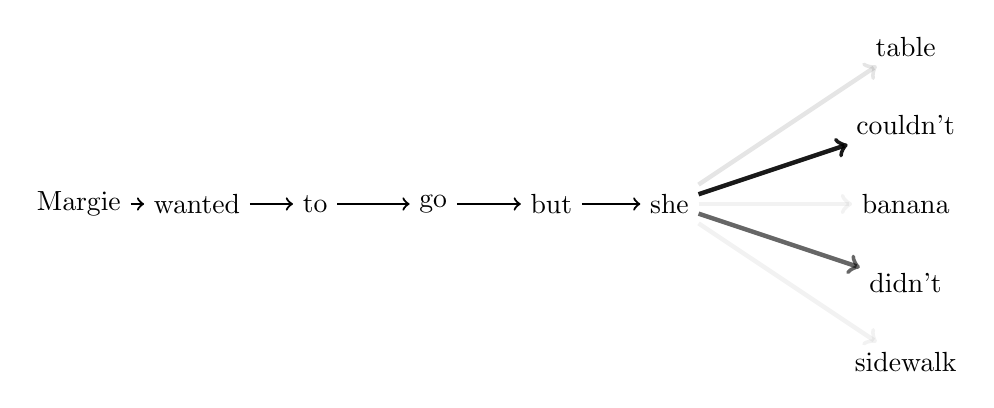
\begin{tikzpicture}[xscale = 1.5]
  \node (W1) at (0, 0) {
    Margie
  };


  \node (W2) at (1, 0) {
    wanted
  };

  \node (W3) at (2, 0) {
    to
  };

  \node (W4) at (3, 0) {
    go
  };

  \node (W5) at (4, 0) {
    but
  };

  \node (W6) at (5, 0) {
    she
  };

  \node (W7) at (7, 2) {
    table
  };

  \node (W8) at (7, 1) {
    couldn't
  };

  \node (W9) at (7, 0) {
    banana
  };

  \node (W10) at (7, -1) {
    didn't
  };

  \node (W11) at (7, -2) {
    sidewalk
  };

  \draw[thick, ->] (W1) -- (W2);
  \draw[thick, ->] (W2) -- (W3);
  \draw[thick, ->] (W3) -- (W4);
  \draw[thick, ->] (W4) -- (W5);
  \draw[thick, ->] (W5) -- (W6);
  \draw[ultra thick, ->, opacity = 0.1] (W6) -- (W7);
  \draw[ultra thick, ->, opacity = 0.9] (W6) -- (W8);
  \draw[ultra thick, ->, opacity = 0.05] (W6) -- (W9);
  \draw[ultra thick, ->, opacity = 0.6] (W6) -- (W10);
  \draw[ultra thick, ->, opacity = 0.05] (W6) -- (W11);
\end{tikzpicture}

  \end{figure}

\end{frame}
%%%%%%%%%%%%%%%%%%%%%%%%%%%%%%%%%%%%%%%%%%%%%%%%%%%%%%%%%%%%%%%%%%%%%%

%%%%%%%%%%%%%%%%%%%%%%%%%%%%%%%%%%%%%%%%%%%%%%%%%%%%%%%%%%%%%%%%%%%%%%
\begin{frame}

  \frametitle{Results on standard datasets}

  New state of the art on the following tasks:

  \bigskip

  \begin{itemize}
  \item Textual Entailment
    \begin{itemize}
      \footnotesize
    \item SNLI $89.3 \rightarrow 89.9$
    \item MNLI Matched $80.6 \rightarrow 82.1$
    \item MNLI Mismatched $80.1 \rightarrow 81.4$
    \item SciTail $83.3 \rightarrow 88.3$
    \item QNLI $82.3 \rightarrow 88.1 $
    \end{itemize}
    \smallskip
  \item Semantic Similarity
    \begin{itemize}
      \footnotesize
    \item STS-B $81.0 \rightarrow 82.0$
    \item QQP $66.1 \rightarrow 70.3$
    \end{itemize}
    \smallskip
  \item Reading Comprehension
    \begin{itemize}
      \footnotesize
    \item RACE $53.3 \rightarrow 59.0$
    \end{itemize}
    \smallskip
  \item Commonsense Reasoning
    \begin{itemize}
      \footnotesize
    \item ROCStories $77.6 \rightarrow 86.5$
    \item COPA $71.2 \rightarrow 78.6$
    \end{itemize}
    \smallskip
  \item Linguistic Acceptability
    \begin{itemize}
      \footnotesize
      \item CoLA $35.0 \rightarrow 45.4$
    \end{itemize}
    \smallskip
  \item Multi-Task Benchmark
    \begin{itemize}
      \footnotesize
      \item GLUE $68.9 \rightarrow 72.8$
    \end{itemize}
  \end{itemize}

\end{frame}
%%%%%%%%%%%%%%%%%%%%%%%%%%%%%%%%%%%%%%%%%%%%%%%%%%%%%%%%%%%%%%%%%%%%%%

%%%%%%%%%%%%%%%%%%%%%%%%%%%%%%%%%%%%%%%%%%%%%%%%%%%%%%%%%%%%%%%%%%%%%%
\begin{frame}
  \frametitle{References}

  \begin{itemize}
  \item Vaswani, Ashish, et al. "Attention is all you need." Advances in Neural Information Processing Systems. 2017.

  \item Radford, Alec, et al. "Improving language understanding by generative pre-training." URL
    \href{https://s3-us-west-2.amazonaws.com/openai-assets/research-covers/language-unsupervised/language_understanding_paper.pdf}{Article pdf link}
    \href{https://blog.openai.com/language-unsupervised/}{Blog post} (2018).

  \item Devlin, Jacob, et al. "BERT: Pre-training of Deep Bidirectional Transformers for Language Understanding." arXiv preprint arXiv:1810.04805 (2018).
  \end{itemize}
\end{frame}
%%%%%%%%%%%%%%%%%%%%%%%%%%%%%%%%%%%%%%%%%%%%%%%%%%%%%%%%%%%%%%%%%%%%%%

\end{document}
